\section*{Appendix}
\begin{comment}
   The appendices contain information
that is peripheral to the main body of the report.
Information typically included are things like
program listings, complex circuit diagrams,
tables, proofs, graphs or any other material
which would break up the theme of the text if it
appeared in situ. Large program listings may be
submitted with the report although it is
preferable either to provide them on CD, or to
cite details of a suitable accessible cloud
repository containing the material. Where CDs
are used you must prepare two CDs, one for each
paper copy of the report.\\ \newline \noindent Please use 
appendices as necessary for material that
is tangentially relevant, or necessary to preserve
project value, but that you do not expect Examiners to
read. Note that software projects with significant code
should normally provide electronic versions of the
code on USB stick, CDROM, or cloud repository. In
that case the Appendix should state where the code
may be found. \textbf{The Appendix should normally
include, or refer to, all the technical details needed
for another user to continue code development}.
Typical items that should not be in the main report,
but should (possibly - since Appendices are not
normally read this is a matter of judgement) be in
appendices:
\begin{itemize}
    \item Source code. Note that code (if long) should
    also be available in some electronic form, e.g. a github repository, CD, or USB 
    stick. Software
    projects must provide access to the source
    code in some form. The Appendix will then
    reference this.
    \item Test data sets (again, for large volumes of
    data an electronic form would be more
    appropriate). The report itself will contain
    concise summaries of the test data in a
    human readable form.
    \item Raw results. Tables of results in unreadable
    form should not be put in the main report, but
    if needed may be put in an Appendix.
    \item Related material possibly but not directly
    relevant to the project work. E.g. manuals of
    test equipment used. (There is no
    requirement to include such, but in some
    cases, where they have some tangential
    relevance, it might be appropriate)
\end{itemize}
 
\end{comment}
\subsection*{FYP Mission Statement (correct to June 2022)}
'\emph{Ambulatory blood pressure monitoring has become increasingly 
relevant due to the advancement of wearable technology. 
Modalities such as Electrocardiogram (ECG) and Photoplethysmography 
(PPG) have provided an indirect method of blood pressure estimations 
compared to a traditional blood-pressure monitor. Although algorithms 
exist for calculating blood pressure with ECG and PPG, it is vital 
that their computational complexity is minimal, whilst maintaining 
accuracy, due to the power limitations of wearable technology. The 
goal of this project is to establish the tradeoffs between using 
PPG and ECG to quantify blood pressure, in the context of wearable
 technology, where power must be kept to a minimum. This project is
  ideal for students interested in signal processing, who have 
  excellent programming skills in Matlab.}'


\subsection*{Health standards requirements for blood pressure estimation}
\begin{itemize}
    \item The Advancement of Medical Instrumentation (AAMI) standard requires a mean BP difference of $\le 5$ mmHg with a standard deviation of $\le 8$ mmHg against auscultatory reference measurement
    \item Significant variation in BP measurements($> 12$ mmHg systolic or $> 8$ mmHg diastolic) from the validated reference device is an exclusion criterion in the AAMI protocol \cite{Bard2019}
    \item The European Society of Hypertension (ESH) protocol requires that the majority of subjects have investigational BP readings within $\le 5$ mmHg of the reference measurement.
\end{itemize}

\subsection*{Complete FYP Gantt chart}

\subsection*{Overview on Cuff-Less BP device options} 
Wearable technology provides an opportunity for real-time monitoring of human vital signs, thus enabling the
 possibility for preventive, timely notification and real-time diagnosis. Unlike commonly-used BP sensors,
  which demand a specific measurement procedure, modern wearable bio-sensors monitor vital signals online and all
   day long, presenting no additional burden other than wearing the device.  A wide range of wearable 
   devices achieve very positive results, even those wearables which are cheaper in price \cite{Simjanoska20182}. Some
    of the systems developed for the purpose of non-invasive BP monitoring will be discussed in more detail now. 
    In addition, they will be critically analysed against two other viable alternatives. \\ \newline \noindent The 
    motivation behind this project is to replace the current cuff-based BP devices. Cuff-based devices often
     require the supervision of an expert to work correctly and do not provide continuous measurements for BP. 
     In addition they can cause irritation and inconvenience for patients due to cuff inflation and deflation. 
     As a result, current clinical cuff-based BP devices are not suitable for providing continuous BP monitoring 
     which could play a significant role in the early detection of diseases which affect the heart \cite{ElHajj2020}.

\subsubsection*{Smart Watches}
Smart watches are becoming an increasingly popular form of wearable technology \cite{Bard2019}. Most of the existing smart
 watch produces currently measure BP through Pulse Transit Time (PTT) from a pulse wave measurement at the wrist. The Heartisans 
 BP smartwatch uses ECG and PPG signals to measure PTT and estimate BP. The watch requires a motionless 20 second scan with 
 the device held at heart level for measurements and provides systolic and diastolic BP readings. Calibration with a
  validated cuff-type BP device is required prior to standalone use. Despite its availability on the market, the 
  Heartisans Watch has not undergone a formal validation study \cite{Bard2019}. \\ \newline \noindent Another wearable 
  method  is  through  arterial  tonometry. The BPro device, developed by the London company HealthSTATS Technologies, 
  is one such device.
\begin{figure}[H]
    \centering
    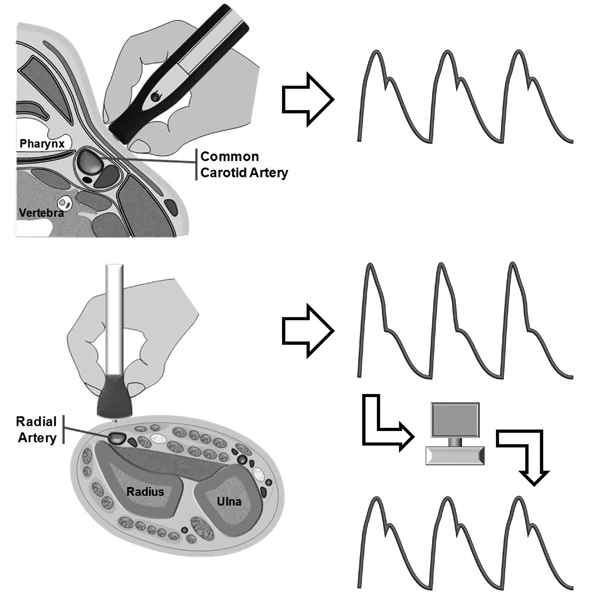
\includegraphics[width=6cm,height=6cm,keepaspectratio]{Background/arterial.png}
    \caption{Arterial Tonometry}
    \label{tonometry}
\end{figure} \noindent Figure \ref{tonometry} shows two different methods for using arterial 
tonometry to measure blood pressure. The first image shows that the recording is taking at the carotid 
artery level in order to estimate the central blood pressure waveform. In the second image, the recording 
is taken at the radial artery level to estimate the arterial pulse wave. The central waveform is then 
reconstructed from this pulse wave using software. \\ \newline \noindent The BPro allows for continuous  24 hour 
 waveform  analysis  of  BP. Calibration to the brachial artery BP is required using a validated upper arm cuff 
 device prior to use. The BPro has been validated in a non-ambulatory study following the Association for the 
 Advancement of Medical Instrumentation (AAMI) standards and the European Society of Hypertension (ESH) protocol.

\subsubsection*{Smartphone Applications}
Smartphones offer a great potential to expand the continuous recording of BP if their sensors can be 
correctly utilised \cite{Bard2019}. A formal validation study on one particular iOS application, the Instant 
Blood Pressure app, revealed poor accuracy of BP measurements. Mean absolute differences of 12.4 mmHg for 
systolic BP and 10.1 mmHg for diastolic BP were found between the Instant Blood Pressure application and a
 reference device. This resulted in approximately four out of five hypertensive individuals being falsely classified 
 as normotensive  \cite{Bard2019}. The My BP Lab application measures BP through measurements of Pulse Transit 
 Time (PTT). However, there is currently a lack of experimental data to justify it's dominance in the market.

\subsubsection*{Medical Tricorders}
A medical tricorder is a handheld portable device used by consumers to self-diagnose medical conditions and take 
basic vital signs measurements. The   BodiMetrics   Performance   Monitor uses ECG and PPG signal data to estimate
 BP through PTT. The Bodimetrics tricorder obtains measurements with a 20 second scan of the user's fingertip
  at heart level but only provides systolic BP data. This tricorder has a large spread in absolute bias against
   an automated sphygmomanometer, hence it is unlikely to meet formal accuracy and precision 
   standards \cite{Bard2019}. \\ \newline \noindent The FreeScan Personal Cardiovascular Monitor, which is 
   developed by the Taiwanese company Maisense Inc., also estimates BP from PTT. However the device uses a force 
   sensor to capture the systolic arterial waveform rather than PPG. This requires the user to physically apply 
   the force sensor directly to the radial artery for around 10 seconds for measurements. The Freescan device 
   has been verified according to the AAMI protocol \cite{Bard2019}. \\ \newline \noindent The SOMNOtouch
    NIBP is a non-traditional medical tricorder that utilizes PTT data collected in a similar fashion to the
     Bodimetrics Performance Monitor. The device has met the ESH standards, however it begins to lose accuracy 
     for higher SBP and DBP values \cite{Bard2019}.

\subsubsection*{Conclusion}
After having discussed three viable devices for cuff-less measurements of BP, it has been finalised that smart 
watches are the most viable option. Whilst existing smart watch devices do suffer from inaccuracies in BP estimation
 due to motion, it is clear that they produce the most acceptable results in line with the AAMI and ESH standards. This 
 chapter can be seen as a forward looking overview of how the estimation methods discussed in this report can be used to
  benefit future products. With regards to this project, this chapter can be treated as a supplementary overview.













\subsection*{Python code for the neural network architectures}
\subsubsection*{AlexNet}
\begin{python}    
    from tensorflow.keras.layers import Softmax, Permute, Input, Add, Conv1D, MaxPooling1D, Dense, Activation, ZeroPadding2D, BatchNormalization, Flatten, Conv2D, AveragePooling1D, MaxPooling2D, GlobalMaxPooling2D, LeakyReLU, GlobalAveragePooling2D, ReLU, Dropout
    from tensorflow.keras.initializers import glorot_uniform
    from tensorflow.keras.models import Model
    import tensorflow as tf
    import scipy
    
    def AlexNet_1D(data_in_shape, num_output=2, dil=1, kernel_size=3, fs = 125, useMaxPooling=True, UseDerivative=False):
    
        # Define the input as a tensor with shape input_shape
        X_input = Input(shape=data_in_shape)
    
        if UseDerivative:
            dt1 = (X_input[:,1:] - X_input[:,:-1])*fs
            dt2 = (dt1[:,1:] - dt1[:,:-1])*fs
            dt1 = tf.pad(dt1, tf.constant([[0,0],[0,1],[0,0]]))
            dt2 = tf.pad(dt2, tf.constant([[0,0],[0,2],[0,0]]))
            X = tf.concat([X_input, dt1, dt2], axis=2)
        else:
            X=X_input
    
    
        # convolutional stage
        X = Conv1D(96, 7, strides=3, name='conv1', kernel_initializer=glorot_uniform(seed=0), padding="same")(X)
        if useMaxPooling:
            X = MaxPooling1D(3, strides=2, name="MaxPool1")(X)
        X = Activation(ReLU())(X)
        X = BatchNormalization(axis=-1, name='BatchNorm1')(X)
    
        X = Conv1D(256, kernel_size=kernel_size, strides=1, dilation_rate=dil, name='conv2', kernel_initializer=glorot_uniform(seed=0), padding="same")(X)
        if useMaxPooling:
            X = MaxPooling1D(3, strides=2, name="MaxPool2")(X)
        X = Activation(ReLU())(X)
        X = BatchNormalization(axis=-1, name='BatchNorm2')(X)
    
        X = Conv1D(384, kernel_size=kernel_size, strides=1, dilation_rate=dil, name='conv3', kernel_initializer=glorot_uniform(seed=0), padding="same")(X)
        X = Activation(ReLU())(X)
        X = BatchNormalization(axis=-1, name='BatchNorm3')(X)
    
        X = Conv1D(384, kernel_size=kernel_size, strides=1, dilation_rate=dil, name='conv4', kernel_initializer=glorot_uniform(seed=0), padding="same")(X)
        X = Activation(ReLU())(X)
        X = BatchNormalization(axis=-1, name='BatchNorm4')(X)
    
        X = Conv1D(256, kernel_size=kernel_size, strides=1, dilation_rate=dil, name='conv5', kernel_initializer=glorot_uniform(seed=0), padding="same")(X)
        if useMaxPooling:
            X = MaxPooling1D(3, strides=2, name="MaxPool5")(X)
        X = Activation(ReLU())(X)
        X = BatchNormalization(axis=-1, name='BatchNorm5')(X)
    
        # Fully connected stage
        X = Flatten()(X)
        X = Dense(4096, activation='relu', name='dense1', kernel_initializer=glorot_uniform(seed=0))(X)
        X = Dropout(rate=0.5)(X)
        X = Dense(4096, activation='relu', name='dense2', kernel_initializer=glorot_uniform(seed=0))(X)
        X = Dropout(rate=0.5)(X)
    
        # Create model
        if num_output == 1:
            X_out = Dense(3, activation='softmax', name='out', kernel_initializer=glorot_uniform(seed=0))(X)
            model = Model(inputs=X_input, outputs=X_out, name='AlexNet_1D')
        else:
            # output stage
            X_SBP = Dense(1, activation='relu', name='SBP', kernel_initializer=glorot_uniform(seed=0))(X)
            X_DBP = Dense(1, activation='relu', name='DBP', kernel_initializer=glorot_uniform(seed=0))(X)
            model = Model(inputs=X_input, outputs=[X_SBP, X_DBP], name='AlexNet_1D')
    
        return model
\end{python}

\subsubsection*{ResNet}
\begin{python}
from tensorflow.keras import layers
from tensorflow.keras.layers import Input, Add, Dense, Activation, ZeroPadding1D, BatchNormalization, Flatten, Conv1D, AveragePooling1D, MaxPooling1D, GlobalMaxPooling2D, LeakyReLU, GlobalAveragePooling2D, ReLU, concatenate
from tensorflow.keras.initializers import glorot_uniform, constant
from tensorflow.keras.models import Model
import tensorflow as tf


def identity_block(X, f, filters, stage, block, dil=1):

    # Implementation of the identity block as defined in Figure 3
    
    # Arguments:
    # X -- input tensor of shape (m, n_H_prev, n_W_prev, n_C_prev)
    # f -- integer, specifying the shape of the middle CONV's window for the main path
    # filters -- python list of integers, defining the number of filters in the CONV layers of the main path
    # stage -- integer, used to name the layers, depending on their position in the network
    # block -- string/character, used to name the layers, depending on their position in the network
    
    #  Returns:
    # X -- output of the identity block, tensor of shape (n_H, n_W, n_C)
    
    # defining name basis
    conv_name_base = 'res' + str(stage) + block + '_branch'
    bn_name_base = 'bn' + str(stage) + block + '_branch'
    
    # Retrieve Filters
    F1, F2, F3 = filters
    
    # Save the input value. You'll need this later to add back to the main path. 
    X_shortcut = X
    
    # First component of main path
    X = Conv1D(filters = F1, kernel_size = 1, strides = 1, dilation_rate=dil, padding = 'valid', name = conv_name_base + '2a', kernel_initializer = glorot_uniform(seed=0))(X)
    X = BatchNormalization(momentum = 0.9, name = bn_name_base + '2a')(X)
    X = Activation(ReLU())(X)

    # Second component of main path
    X = Conv1D(filters = F2, kernel_size = f, strides = 1, dilation_rate=dil, padding = 'same', name = conv_name_base + '2b', kernel_initializer = glorot_uniform(seed=0))(X)
    X = BatchNormalization(momentum=0.9, name=bn_name_base + '2b')(X)
    X = Activation(ReLU())(X)

    # Third component of main path
    X = Conv1D(filters = F3, kernel_size = 1, strides = 1, dilation_rate=dil, padding = 'valid', name = conv_name_base + '2c', kernel_initializer = glorot_uniform(seed=0))(X)
    X = BatchNormalization(momentum = 0.9, name = bn_name_base + '2c')(X)

    # Final step: Add shortcut value to main path, and pass it through a RELU activation
    X = Add()([X, X_shortcut])
    X = Activation(ReLU())(X)
    # X = BatchNormalization(momentum = 0.9, name = bn_name_base + '2c')(X)
    
    return X

def convolutional_block(X, f, filters, stage, block, s = 2, dil = 1):

    # Implementation of the convolutional block as defined in Figure 4
    
    # Arguments:
    # X -- input tensor of shape (m, n_H_prev, n_W_prev, n_C_prev)
    # f -- integer, specifying the shape of the middle CONV's window for the main path
    # filters -- python list of integers, defining the number of filters in the CONV layers of the main path
    # stage -- integer, used to name the layers, depending on their position in the network
    # block -- string/character, used to name the layers, depending on their position in the network
    # s -- Integer, specifying the stride to be used
    
    # Returns:
    # X -- output of the convolutional block, tensor of shape (n_H, n_W, n_C)
    
    # defining name basis
    conv_name_base = 'res' + str(stage) + block + '_branch'
    bn_name_base = 'bn' + str(stage) + block + '_branch'
    
    # Retrieve Filters
    F1, F2, F3 = filters
    
    # Save the input value
    X_shortcut = X


    ##### MAIN PATH #####
    # First component of main path 
    X = Conv1D(F1, 1, strides = s, name = conv_name_base + '2a', kernel_initializer = glorot_uniform(seed=0))(X)
    X = BatchNormalization(momentum=0.9, name=bn_name_base + '2a')(X)
    X = Activation(ReLU())(X)
    
    # Second component of main path
    X = Conv1D(filters = F2, kernel_size = f, strides = 1, dilation_rate=dil, padding = 'same', name = conv_name_base + '2b', kernel_initializer = glorot_uniform(seed=0))(X)
    X = BatchNormalization(momentum=0.9, name=bn_name_base + '2b')(X)
    X = Activation(ReLU())(X)

    # Third component of main path
    X = Conv1D(filters = F3, kernel_size = 1, dilation_rate=dil, strides = 1, padding = 'valid', name = conv_name_base + '2c', kernel_initializer = glorot_uniform(seed=0))(X)
    X = BatchNormalization(momentum = 0.9, name = bn_name_base + '2c')(X)

    ##### SHORTCUT PATH ####
    X_shortcut = Conv1D(filters = F3, kernel_size = 1, strides = s, padding = 'valid', name = conv_name_base + '1',
                        kernel_initializer = glorot_uniform(seed=0))(X_shortcut)
    X_shortcut = BatchNormalization( momentum = 0.9, name = bn_name_base + '1')(X_shortcut)

    # Final step: Add shortcut value to main path, and pass it through a RELU activation
    X = Add()([X, X_shortcut])
    X = Activation(ReLU())(X)
    # X = BatchNormalization(momentum = 0.9, name = bn_name_base + '2c')(X)
    
    return X

def ResNet50_1D(data_in_shape, num_output=2, fs=125, UseDerivative=False):

    # Implementation of the popular ResNet50 the following architecture:
    # CONV2D -> BATCHNORM -> RELU -> MAXPOOL -> CONVBLOCK -> IDBLOCK*2 -> CONVBLOCK -> IDBLOCK*3
    # -> CONVBLOCK -> IDBLOCK*5 -> CONVBLOCK -> IDBLOCK*2 -> AVGPOOL -> TOPLAYER

    # Arguments:
    # input_shape -- shape of the images of the dataset
    # classes -- integer, number of classes
    # Returns:
    # model -- a Model() instance in Keras

    # Define the input as a tensor with shape input_shape
    X_input = Input(shape=data_in_shape)

    if UseDerivative:
        dt1 = (X_input[:,1:] - X_input[:,:-1])*fs
        dt2 = (dt1[:,1:] - dt1[:,:-1])*fs

        dt1 = tf.pad(dt1, tf.constant([[0,0],[0,1],[0,0]]))
        dt2 = tf.pad(dt2, tf.constant([[0,0],[0,2],[0,0]]))

        X = tf.concat([X_input, dt1, dt2], axis=2)
    else:
        X=X_input

    # Zero-Padding
    X = ZeroPadding1D(3)(X_input)

    # Stage 1
    X = Conv1D(64, 7, strides=2, name='conv1', kernel_initializer=glorot_uniform(seed=0))(X)
    X = BatchNormalization(axis=2, name='bn_conv1')(X)
    X = Activation('relu')(X)
    X = MaxPooling1D(3, strides=3)(X)

    # Stage 2
    X = convolutional_block(X, f=3, filters=[64, 64, 256], stage=2, block='a', s=1)
    X = identity_block(X, 3, [64, 64, 256], stage=2, block='b')
    X = identity_block(X, 3, [64, 64, 256], stage=2, block='c')

    # Stage 3
    X = convolutional_block(X, f = 3, filters = [128, 128, 512], stage = 3, block='a', s = 2)
    X = identity_block(X, 3, [128, 128, 512], stage=3, block='b')
    X = identity_block(X, 3, [128, 128, 512], stage=3, block='c')
    X = identity_block(X, 3, [128, 128, 512], stage=3, block='d')

    # Stage 4
    X = convolutional_block(X, f = 3, filters = [256, 256, 1024], stage = 4, block='a', s = 2)
    X = identity_block(X, 3, [256, 256, 1024], stage=4, block='b')
    X = identity_block(X, 3, [256, 256, 1024], stage=4, block='c')
    X = identity_block(X, 3, [256, 256, 1024], stage=4, block='d')
    X = identity_block(X, 3, [256, 256, 1024], stage=4, block='e')
    X = identity_block(X, 3, [256, 256, 1024], stage=4, block='f')

    # Stage 5
    X = convolutional_block(X, f = 3, filters = [512, 512, 2048], stage = 5, block='a', s = 2)
    X = identity_block(X, 3, [512, 512, 2048], stage=5, block='b')
    X = identity_block(X, 3, [512, 512, 2048], stage=5, block='c')

    X = AveragePooling1D(2, name="avg_pool")(X)

    # output layer
    X = Flatten()(X)
    X_SBP = Dense(1, activation='linear', name='SBP', kernel_initializer = glorot_uniform(seed=0))(X)
    X_DBP = Dense(1, activation='linear', name='DBP', kernel_initializer = glorot_uniform(seed=0))(X)
    HR = Dense(1, activation='linear', name='HR', kernel_initializer = glorot_uniform(seed=0))(X)
    
    # Create model
    if num_output==3:
        model = Model(inputs=X_input, outputs=[X_SBP, X_DBP, HR], name='ResNet50_1D')
    else:
        model = Model(inputs = X_input, outputs = [X_SBP, X_DBP], name='ResNet50_1D')

    return model
\end{python}

\subsubsection*{ResNet with Leave One Subject Out (LOSO)}
\begin{python}
from __future__ import division, print_function
import numpy as np
np.random.seed(3)
import os

from scipy.signal import butter, lfilter, lfilter_zi, filtfilt, savgol_filter
from sklearn.preprocessing import MinMaxScaler
import sklearn as sk
import random
random.seed(3)

import scipy.io as sio
import matplotlib.pyplot as plt
import natsort as natsort
from scipy import signal
import math

import tensorflow as tf
# from tensorflow.keras.utils import multi_gpu_model

from tensorflow.keras.models import Sequential
from tensorflow.keras.backend import squeeze
from kapre import STFT, Magnitude, MagnitudeToDecibel
# from kapre.utils import Normalization2D
from tensorflow.keras.layers import Input, BatchNormalization, Lambda, AveragePooling2D, Flatten, Dense, Conv1D, Activation, add, AveragePooling1D, Dropout, Permute, concatenate, MaxPooling1D, LSTM, Reshape, GRU
from tensorflow.keras.regularizers import l2
from tensorflow.keras import Model
from tensorflow.keras import optimizers
#from tensorflow.keras.utils.vis_utils import plot_model

from tensorflow.keras.layers import Conv2D, MaxPooling2D

def diff(input, fs):
    dt = (input[:, 1:] - input[:, :-1]) * fs
    dt = tf.pad(dt, tf.constant([[0, 0], [0, 1], [0, 0]]))

    return dt

def mid_spectrogram_layer(input_x):
    l2_lambda = .001
    n_dft = 128
    n_hop = 64
    fmin = 0.0
    fmax = 50 / 2

    x = Permute((2, 1))(input_x)
    # x = input_x
    x = STFT(n_fft=n_dft, hop_length=n_hop, output_data_format='channels_last')(x)
    x = Magnitude()(x)
    #x = MagnitudeToDecibel()(x)
    #x = BatchNormalization()(x)
    # x = Normalization2D(str_axis='batch')(x)
    x = Flatten()(x)
    x = Dense(32, activation="relu", kernel_regularizer=l2(l2_lambda))(x)
    x = BatchNormalization()(x)

    return x


def mid_spectrogram_LSTM_layer(input_x):
    l2_lambda = .001
    n_dft = 64

    n_hop = 64
    fmin = 0.0
    fmax = 50 / 2

    #x = Permute((2, 1))(input_x)
    x = input_x
    x = STFT(n_fft=n_dft, hop_length=n_hop, output_data_format='channels_last')(x)
    x = Magnitude()(x)
    x = MagnitudeToDecibel()(x)
   #x = BatchNormalization()(x)
    # x = Normalization2D(str_axis='batch')(x)
    # print(np.array(x).shape)
    # x = Reshape((2, 64))(x)
    # x = GRU(64)(x)
    x = Flatten()(x)
    x = Dense(32, activation="relu", kernel_regularizer=l2(l2_lambda))(x)
    x = BatchNormalization()(x)

    return x


def single_channel_resnet(my_input, num_filters=64, num_res_blocks=4, cnn_per_res=3,
                          kernel_sizes=[8, 5, 3], max_filters=128, pool_size=3, pool_stride_size=2):

    #my_input = Input(shape=input_shape)
    # my_input = input_shape
    # my_input = ks.expand_dims(my_input, axis=2)

    for i in np.arange(num_res_blocks):
        if (i == 0):
            block_input = my_input
            x = BatchNormalization()(block_input)
        else:
            block_input = x

        for j in np.arange(cnn_per_res):
            x = Conv1D(num_filters, kernel_sizes[j], padding='same')(x)
            x = BatchNormalization()(x)
            if (j < cnn_per_res - 1):
                x = Activation('relu')(x)

        is_expand_channels = not (my_input.shape[0] == num_filters)

        if is_expand_channels:
            res_conn = Conv1D(num_filters, 1, padding='same')(block_input)
            res_conn = BatchNormalization()(res_conn)
        else:
            res_conn = BatchNormalization()(block_input)

        x = add([res_conn, x])
        x = Activation('relu')(x)

        if (i < 5):
            x = AveragePooling1D(pool_size=pool_size, strides=pool_stride_size)(x)

        num_filters = 2 * num_filters
        if max_filters < num_filters:
            num_filters = max_filters

    return my_input, x


def raw_signals_deep_ResNet(input, UseDerivative=False):
    fs=125

    inputs = []
    l2_lambda = .001
    channel_outputs = []
    num_filters = 32

    X_input = Input(shape=input)

    if UseDerivative:
        # fs = tf.constant(fs, dtype=float)
        X_dt1 = Lambda(diff, arguments={'fs': fs})(X_input)
        X_dt2 = Lambda(diff, arguments={'fs': fs})(X_dt1)
        X = [X_input, X_dt1, X_dt2]
    else:
        X = [X_input]

    num_channels = len(X)

    for i in np.arange(num_channels):
        channel_resnet_input, channel_resnet_out = single_channel_resnet(X[i], num_filters=num_filters,
        num_res_blocks=4, cnn_per_res=3, kernel_sizes=[8, 5, 5, 3], max_filters=64, pool_size=2, pool_stride_size=1)
        channel_outputs.append(channel_resnet_out)
        inputs.append(channel_resnet_input)

    spectral_outputs = []
    num_filters = 32
    for x in inputs:
        spectro_x = mid_spectrogram_LSTM_layer(x)
        spectral_outputs.append(spectro_x)

    # concatenate the channel specific residual layers

    # print("Num Channels: ", num_channels)

    if num_channels > 1:
        x = concatenate(channel_outputs, axis=-1)
    else:
        x = channel_outputs[0]

    x = BatchNormalization()(x)
    x = GRU(65)(x)
    # x = Flatten()(x)
    x = BatchNormalization()(x)

    # join time-domain and frequnecy domain fully-conencted layers
    if num_channels > 1:
        s = concatenate(spectral_outputs, axis=-1)
    else:
        s = spectral_outputs[0]

    # s = Flatten()(s)
    #     x = Dense(128,activation="relu",kernel_regularizer=l2(l2_lambda)) (x)
    s = BatchNormalization()(s)
    # LETS DO OVERFIT
    x = concatenate([s, x])
    x = Dense(32, activation="relu", kernel_regularizer=l2(l2_lambda))(x)
    x = Dropout(0.25)(x)
    x = Dense(32, activation="relu", kernel_regularizer=l2(l2_lambda))(x)
    x = Dropout(0.25)(x)
    #output = Dense(2, activation="relu")(x)
    x = Flatten()(x)
    X_SBP = Dense(1, activation='linear', name='SBP')(x)
    X_DBP = Dense(1, activation='linear', name='DBP')(x)

    model = Model(inputs=X_input, outputs=[X_SBP, X_DBP], name="Slapnicar_Model")
    # model = multi_gpu_model(model, gpus=2)
    # optimizer = optimizers.Adadelta()
    # loss = ks.keras.losses.mean_absolute_error
    # model.compile(optimizer=optimizer, loss=loss, metrics=['mae', 'mae'])
    print(model.summary())
    # plot_model(model=model, to_file='lstm_model.png', show_shapes=True, show_layer_names=True)
    return model


def one_chennel_resnet(input_shape,num_filters=16,num_res_blocks = 5,cnn_per_res = 3,
                        kernel_sizes = [3,3,3], max_filters = 64, pool_size = 3,
                        pool_stride_size = 2,num_classes=8):
    my_input  = Input(shape=(input_shape))
    for i in np.arange(num_res_blocks):
        if(i==0):
            block_input = my_input
            x = BatchNormalization()(block_input)
        else:
            block_input = x
        for j in np.arange(cnn_per_res):
            x = Conv1D(num_filters, kernel_sizes[j], padding='same')(x)
            x = BatchNormalization()(x)
            if(j<cnn_per_res-1):
                x = Activation('relu')(x)
        is_expand_channels = not (input_shape[0] == num_filters)
        if is_expand_channels:
            res_conn = Conv1D(num_filters, 1,padding='same')(block_input)
            res_conn = BatchNormalization()(res_conn)
        else:
            res_conn = BatchNormalization()(block_input)
        x = add([res_conn, x])
        x = Activation('relu')(x)
        if(i<5):
            x = MaxPooling1D(pool_size=pool_size,strides =pool_stride_size)(x)
        num_filters = 2*num_filters
        if max_filters<num_filters:
            num_filters = max_filters
    return my_input,x


def one_chennel_resnet_2D(input_shape, input_layer, num_filters=16,num_res_blocks = 5,cnn_per_res = 3,
                        kernel_sizes = [8, 5, 3], max_filters = 64, pool_size = (3,3),
                        pool_stride_size = 2, num_classes=8):
    kernel_sizes = [(8, 1), (5, 1), (3, 1)]
    my_input = input_layer
    for i in np.arange(num_res_blocks):
        if(i==0):
            block_input = my_input
            x = BatchNormalization()(block_input)
        else:
            block_input = x
        for j in np.arange(cnn_per_res):
            x = Conv2D(num_filters, kernel_sizes[j], padding='same')(x)
            x = BatchNormalization()(x)
            if(j<cnn_per_res-1):
                x = Activation('relu')(x)
        is_expand_channels = not (input_shape[0] == num_filters)
        if is_expand_channels:
            res_conn = Conv2D(num_filters, (1,1), padding='same')(block_input)
            res_conn = BatchNormalization()(res_conn)
        else:
            res_conn = BatchNormalization()(block_input)
        x = add([res_conn, x])
        x = Activation('relu')(x)
        if(i<5):
            x = MaxPooling2D(pool_size=pool_size,strides =pool_stride_size)(x)
        num_filters = 2*num_filters
        if max_filters<num_filters:
            num_filters = max_filters
    return my_input,x


def spectro_layer_mid(input_x,sampling_rate, ndft=0, num_classes=8):
    l2_lambda = .001
    if(ndft == 0):
        n_dft= 128
    else:
        n_dft = ndft
    # n_dft = 64
    n_hop = 64
    fmin=0.0
    fmax=sampling_rate//2

    x = Permute((2,1))(input_x)
    x = STFT(n_fft=n_dft, hop_length=n_hop, output_data_format='channels_last')(x)
    x = Magnitude()(x)
    #x = MagnitudeToDecibel()(x)
    #x = BatchNormalization()(x)    # x = Normalization2D(str_axis='batch')(x)
    channel_resnet_input,channel_resnet_out= one_chennel_resnet_2D((625, 1), x, num_filters=64,
                    num_res_blocks = 6,cnn_per_res = 3,kernel_sizes = [3,3,3,3],
                    max_filters = 32, pool_size = 1,
                    pool_stride_size =1,num_classes=8)
    channel_resnet_out = BatchNormalization()(channel_resnet_out)

    # x = Reshape((10, 65))(x)
    # x = GRU(65)(x)

    return channel_resnet_out
\end{python}

\subsubsection*{LSTM}

\begin{python}
    from tensorflow.keras.layers import Input, LSTM, Dense, Bidirectional, Conv1D, ReLU

from tensorflow.keras import Model

def define_LSTM(data_in_shape, UseDerivative=False):
    X_input = Input(shape=data_in_shape)

    fs = 125

    if UseDerivative:
        dt1 = (X_input[:,1:] - X_input[:,:-1])*fs
        dt2 = (dt1[:,1:] - dt1[:,:-1])*fs

        dt1 = tf.pad(dt1, tf.constant([[0,0],[0,1],[0,0]]))
        dt2 = tf.pad(dt2, tf.constant([[0,0],[0,2],[0,0]]))

        X = tf.concat([X_input, dt1, dt2], axis=2)
    else:
        X=X_input


    X = Conv1D(filters=64, kernel_size=5, strides=1, padding='causal', activation='relu')(X)
    X = Bidirectional(LSTM(128, return_sequences=True))(X)
    X = Bidirectional(LSTM(128, return_sequences=True))(X)
    X = Bidirectional(LSTM(64, return_sequences=False))(X)
    X = Dense(512, activation='relu')(X)
    X = Dense(256, activation='relu')(X)
    X = Dense(128, activation='relu')(X)

    X_SBP = Dense(1, name='SBP')(X)
    X_DBP = Dense(1, name='DBP')(X)

    model = Model(inputs=X_input, outputs=[X_SBP, X_DBP], name='LSTM')

    return model
\end{python}

\subsubsection*{Transformer encoder}
\begin{python}
from tensorflow import keras
from tensorflow.keras import layers

def transformer_encoder(inputs, head_size, num_heads, ff_dim, dropout=0):
    # Normalization and Attention
    x = layers.LayerNormalization(epsilon=1e-6)(inputs)
    x = layers.MultiHeadAttention(
        key_dim=head_size, num_heads=num_heads, dropout=dropout
    )(x, x)
    x = layers.Dropout(dropout)(x)
    res = x + inputs

    # Feed Forward Part
    x = layers.LayerNormalization(epsilon=1e-6)(res)
    x = layers.Conv1D(filters=ff_dim, kernel_size=1, activation="relu")(x)
    x = layers.Dropout(dropout)(x)
    x = layers.Conv1D(filters=inputs.shape[-1], kernel_size=1)(x)
    return x + res


def define_encoder(
    input_shape,
    head_size,
    num_heads,
    ff_dim,
    num_transformer_blocks,
    mlp_units,
    dropout=0,
    mlp_dropout=0,
    UseDerivative=False
):
    inputs = keras.Input(shape=input_shape)
    X_input = inputs
    fs = 125

    if UseDerivative:
        dt1 = (X_input[:,1:] - X_input[:,:-1])*fs
        dt2 = (dt1[:,1:] - dt1[:,:-1])*fs

        dt1 = tf.pad(dt1, tf.constant([[0,0],[0,1],[0,0]]))
        dt2 = tf.pad(dt2, tf.constant([[0,0],[0,2],[0,0]]))

        x = tf.concat([X_input, dt1, dt2], axis=2)
    else:
        x=X_input

    for _ in range(num_transformer_blocks):
        x = transformer_encoder(x, head_size, num_heads, ff_dim, dropout)

    x = layers.GlobalAveragePooling1D(data_format="channels_first")(x)
    for dim in mlp_units:
        x = layers.Dense(dim, activation="relu")(x)
        x = layers.Dropout(mlp_dropout)(x)
    
    # outputs = layers.Dense(1)(x)

    X_SBP = layers.Dense(1, name='SBP')(x)
    X_DBP = layers.Dense(1, name='DBP')(x)

    model = Model(inputs=inputs, outputs=[X_SBP, X_DBP], name='Encoder')
    # return keras.Model(inputs, outputs)
    return model
\end{python}
